% !Mode:: "TeX:UTF-8"
% !TEX root = ..\main.tex
\chapter{冠状动脉切割几种方法的实质和实现}
\section{水平集方法}
水平集方法的原理和实现
\section{mean-shift方法}
Mean Shift是Fukunage提出的一种方法\cite{Cheng1995Mean},由Yizong等人改进\cite{Cheng1995Mean}。



均值偏移把特征空间当做经验概率密度函数。如果输入是点的集合,均值偏移考虑这些点是从潜在的概率密度函数中提取出来的。如果稠密的区域出现在特征空间中,它们就是潜在的概率密度函数的模式。我们使用均值
偏移识别出和固定模式相关联的簇。对于每一个数据点,均值偏移以这个点为中心定义了一个窗口,计算这个窗口内数据点的平均值。然后移动窗口的中心到平均值处,重复整个算法过程直到收敛。在每一次迭代后,我们
认为窗口移动到数据更密集的区域。

抽象概括来说,我们可以描述均值偏移的过程如下:
\begin{enumerate}
  \item 以每个数据点为中心确定一个窗口
  \item 计算窗口区域内数据点的平均值
  \item 移动窗口,重复这个过程直到收敛
\end{enumerate}
\subsection{核函数}
一个函数是核函数,需要满足如下两个要求

\begin{enumerate}
  \item $\int_{R^d} \phi (x) dx = 1$
  \item $\phi (x) \geq 0 $
\end{enumerate}
举几个常见核函数的例子

Rectangular核函数
\begin{equation}\label{eq:kernel_rectangular}
\phi (x)=\left\{
\begin{aligned}
 1  && {a \leq x \leq b} \\
 0  && {else}
\end{aligned}
\right.
\end{equation}

最常见的是高斯核函数
\begin{align}\label{eq:kernel_guassian}
	\phi (x) = e^{-\frac{x^{2}}{2\sigma^2}}
\end{align}

还有Epanechnikov核函数
\begin{equation}\label{eq:kernel_rectangular}
\phi (x)=\left\{
\begin{aligned}
 \frac{3}{4}(1-x^{2})  && {if \left| x \right| \leq 1} \\
 0  && {else}
\end{aligned}
\right.
\end{equation}

\subsection{核函数密度估计}
核函数密度估计是一种估计随机变量密度函数的非参数方式。它经常被称作Parzen窗口技术。给定一个函数,步长h,核密度估计对一个多维集合点来说是
\begin{align}\label{eq:parzen_window}
	\hat{f}(x) = \frac{1}{nh^d}\sum_{i=1}^{n}K(\frac{x-x_{i}}{h})
\end{align}

\subsection{均值偏移的梯度上升}
均值偏移是基于密度轮廓的梯度上升。梯度上升的通常形式
\begin{align}\label{eq:gradient_ascent}
	x_{1} = x_{0} + \eta f^{'}(x_{0})
\end{align}
我们把梯度上升运用到\eqref{eq:parzen_window}得到梯度
\begin{align}\label{eq:eq:parzen_window_gradient}
	\nabla \hat{f}(x)= \frac{1}{h^{d+1}}\sum K^{'}(\frac{x-x_{i}}{h})
\end{align}
我们把梯度设为0,我们得到
\begin{align}\label{eq:parzen_window_gradient}
\sum_{i=1}^{n}K^{'}(\frac{x-x_{i}}{h})\vec{x} = \sum_{i=1}^{n}K^{'}(\frac{x-x_{i}}{h})\vec{x_{i}}
\end{align}
最后我们得到,我们得到
\begin{align}\label{eq:original_mean_shift_vector}
\vec{x} =
\frac{\sum_{i=1}^{n}K^{'}(\frac{x-x_{i}}{h})\vec{x_{i}}}{\sum_{i=1}^{n}K^{'}(\frac{x-x_{i}}{h})}
\end{align}

\subsection{偏移}
如前所述,均值偏移把这些点组成的特征空间当做概率密度函数。特征空间中密集的区域对应于最大值,或者就是概率分布的模式。对于每一个点,在局部估计密度运用梯度上升,直到收敛。通过梯度上升得到的
固定的点代表概率密度函数模式。所有属于一个固定点的点组成一个簇,我们假设$g(x) = -K^{'}(x) $,我们有
\begin{align}\label{eq:mean_shift_mx}
m(x) =
\frac{\sum_{i=1}^{n}g(\frac{x-x_{i}}{h})x_{i}}{\sum_{i=1}^{n}g(\frac{x-x_{i}}{h})}
- x
\end{align}

我们把数量$m(x)$叫做均值偏移。把前面迭代过程结合公司描述一下
\begin{enumerate}
  \item 计算均值偏移向量$m(x_{i}^{t}) $
  \item 沿着$m(x_{i}^t)$移动密度估计窗口
  \item 重复这个过程直到收敛
\end{enumerate}
\section{snake方法}
\subsection{snake模型}
1987年Kass等人提出动态轮廓模型\cite{kass1988snakes},这个模型的提出主要是为了找数字图像中的
凸出轮廓,像物体的边界。动态轮廓模型被用于图像的切割和理解,也可以用于动态图像数据
的分析,例如运动跟踪。Kass等人\cite{kass1988snakes}的这篇文章给出了动态轮廓模型的基础,描述了蛇模型的基础等式。其他变种的蛇模型都是以
Kass的这个蛇模型为基础的。他的这个蛇模型也被称为经典蛇模型。
\subsubsection{蛇模型的参数化表示}
蛇模型被定义为能量最小化的样条,它的能量取决于它的形状和它在图像中的位置。蛇模型刚开始的时候形状和在图像中的
位置可以是任意的,然后演化成目标形状,移动到想要的位置和物体的边界或者边缘对齐。蛇模型的演化和移动受到最小化能量的内在趋势激活。当蛇模型和图像中目标物体的边界对齐时,它的能量达到局部最小值。

在\cite{kass1988snakes}中,蛇模型的参数化形式如下:
\begin{align}\label{eq:base_snake_parameter_representation}
	v(s) = [x(s),y(s)],s \in [0,1]
\end{align}

在上面公式中,$x(s),y(s)$是轮廓上各个点的$x,y$坐标,$s$代表弧长,$s$的范围是$[0,1]$。

曲线上每一点的移动,都是为了最小化蛇模型能量函数,它由三个能量成分组成:
\begin{align}\label{eq:base_snake_calculative_representation}
	E = \int_0^1E_{int}(v(s))+E_{image}(v(s))+E_{con}(v(s)) ds
\end{align}

在上面公式中,$E_{int}$代表内在能量,$E_{image}$代表图像能量,$E_{con}$代表外部能量。

\subsubsection{内部能量}
蛇模型每一点的内部能量按照如下方式定义
\begin{align}\label{eq:base_snake_calculative_internal_representation}
	E_{int} = \frac{1}{2}(\alpha|v^{'}(s)|^{2}+\beta|v^{''}(s)|^{2})
\end{align}

在上面公式中$v^{'}(s)=\frac{dv(s)}{ds}$定义了某点沿着切线方向的形变;公式$v^{''}(s)=\frac{d^{2}v(s)}{ds^{2}}$中的定义了某点处曲率的形变。
$\alpha,\beta$是权重系数,各自控制蛇模型的伸缩和弯曲。$\alpha$是伸缩系数,$\beta$是强直系数。


我们很容易找到一种物质用作类比蛇模型,它就是橡皮筋,橡皮筋既能拉长也能弯曲。蛇模型的内部能量是所有点按照公式\eqref{eq:base_snake_calculative_internal_representation}
求出的能量的积分,为了方便解释内部能量又被分成两部分。\eqref{eq:base_snake_calculative_internal_representation}的第一部分被称作伸缩能量,第二部分称作弯曲能量。对它们各自进行
积分得到整个蛇模型的伸缩能量和弯曲能量。

\begin{align}\label{eq:base_snake_calculative_internal_elastic_representation}
	E_{elastic} = \frac{1}{2}\int\alpha(s)|v^{'}(s)|^{2}ds
\end{align}

\begin{align}\label{eq:base_snake_calculative_internal_bending_representation}
	E_{elastic} = \frac{1}{2}\int\beta(s)|v^{''}(s)|^{2}ds
\end{align}

通常来说,$\alpha(s)$和$\beta(s)$在蛇模型中对每一点来说是一样的,就是可以被当作常量。可以用\eqref{eq:base_snake_calculative_internal_elastic_representation}
和\eqref{eq:base_snake_calculative_internal_bending_representation}的最小值解释蛇模型的形变趋势。

(1)伸缩力量:

公式\eqref{eq:base_snake_calculative_internal_elastic_representation}达到最小值,当$v^{'}(s)=0$或者$v(s)=const$,也就是蛇模型的每一点在同一位置。换句话
说,换句话说伸缩力量使得蛇模型变成一个点。

(2)弯曲力量:

公式\eqref{eq:base_snake_calculative_internal_bending_representation}达到最小值,当$v^{''}=0$,这也意味着:
\begin{align}\label{eq:simple_vs_function}
	v(s) = cs
\end{align}

公式\eqref{eq:simple_vs_function}是线性等式。从几何上来说,$v^{''}(s)=0$代表着蛇模型的曲率。所以蛇模型在曲率值高的地方尽量演变成一条直线或者磨平尖角。

\begin{figure}[htbp]
	\centering
	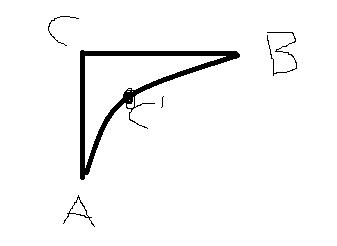
\includegraphics[width=0.5\linewidth]{snakesSmoothOverSharpCorner.png}
	\caption{蛇模型尖角处平滑}\label{fig:snakesSmoothOverSharpCorner}
\end{figure}

在图\ref{fig:snakesSmoothOverSharpCorner}中,点$C$的曲率比$C^{'}$的高。我们假设$AC^{'}B$的半径和$ACB$的半径一样。因为$AC+BC$的弧长比$AC^{'}B$长,
所以点$C$的曲率比点$C^{'}$的曲率高。

\subsubsection{图像能量}
图像能量$E_{image}(v(s))$是从图像推导出来的信息,它对感兴趣的特征区域会采用比较小的值,例如边界。觉个例子,给出一张灰度图像I(x,y),蛇模型是靠近物体边界的,因为在边界处有较大的
梯度值,以及较小的图像能量。
\begin{align}\label{eq:base_snake_image_energy_grey_level_representation}
	E_{image} = -|\nabla I(x,y)|^{2}
\end{align}

但是更常见的是图像能量被定义为另外一种情况:
\begin{align}\label{eq:base_snake_image_energy_grey_level_guassian_representation}
E_{image} = -|\nabla G_{\sigma}(x,y) *  \nabla I(x,y)|^{2}
\end{align}
其中$G_{\sigma}(x,y)$标准差是$\sigma$的二维高斯函数,符号$\nabla$是梯度算子

高斯函数的一个效果是边界被模糊或扩张,这导致蛇模型局部最小值较差的收敛性,好处是我们能从较远的地方使蛇模型靠近最小值。较大的标准差会使捕获空间比较大。在\cite{kass1988snakes}中,
\eqref{eq:base_snake_image_energy_grey_level_representation}叫作边缘函数,而\eqref{eq:base_snake_image_energy_grey_level_guassian_representation}被叫作尺度空间。

\subsubsection{约束能量}
约束能量$E_{con}(v(s))$是一种外部力量,主要是一种相互作用的能量。这种力量是基于高阶约束(这种高阶约束和全局策略相关),例如和图像中其他物体的关系,这种强制力量会迫使蛇模型朝向或者原理特殊区域。它提供了一种外部
约束的度量方式,无论是形状信息还是使用通过交互提供的能量值。


\subsection{snake模型数值解法}
\subsubsection{有限差分法}
snake方法的原理和实现
蛇模型被离散化成N个不同的点,蛇模型的能量\eqref{eq:base_snake_calculative_representation}N个点能量的累积和。
\begin{align}\label{eq:snake_energy_discrete_representation}
E_{snake}^{*} = \sum_{i=1}^{N}E_{int}(i)+E_{ext}(i)
\end{align}

在公式\eqref{eq:base_snake_parameter_representation},参数用$i*h$代替,这里h是固定的步长。
\begin{align}\label{eq:snake_parameter_discrete_representation}
v(s)=v(i)=(x_{i},y_{i})=(x(i*h),y(i*h)) (i=1 \ldots n)
\end{align}

内部能量范围内有限差分的近似导数
\begin{align}\label{eq:simple_parameter_derivative_first_order}
\frac{dv(s)}{ds} = \frac{|v_{i}-v_{i-1}|^{2}}{h^{2}}
\end{align}

\begin{align}\label{eq:simple_parameter_derivative_second_order}
\frac{d^{2}v(s)}{ds^{2}} = \frac{|v_{i+1}-2v_{i}+v_{i-1}|^{2}}{h^{4}}
\end{align}

让$f_{x}(i)=\frac{\partial E_{ext}}{\partial x_{i}}$和$f_{y}(i)=\frac{\partial
E_{ext}}{\partial
y_{i}}$。我们最小化公式\eqref{eq:snake_energy_discrete_representation}等于解下面的欧拉等式:
\begin{align}\label{eq:solve_euler_equations}
\begin{split}
\alpha_{i}[v_{i}-v_{i-1}] - \alpha_{i+1}[v_{i+1} -v_{i}]
+\beta_{i-1}[v_{i-2}-2v_{i-1}+v_{i}]\\
-2\beta_{i}[v_{i-1}-2v_{i}+v_{i+1}]+\beta_{i+1}[v_{i}-2v_{i+1}+v_{i+2}]+(f_{x}(i),f_{y}(i))=0
\end{split}
\end{align}
解决这个等式可以把矩阵运用到\eqref{eq:snake_energy_discrete_representation},这个等式现在是由N个形如\eqref{eq:solve_euler_equations}的欧拉等式组成。
\begin{align}\label{eq:snake_discrete_matrix_form}
\begin{split}
AX+f_{x}(X,Y)=0\\
AY+f_{y}(X,Y)=0
\end{split}
\end{align}
为了解决公式\eqref{eq:snake_discrete_matrix_form},等式的右边设置成步长和左边函数导数的积
\begin{align}\label{eq:snake_discrete_matrix_form_solve}
\begin{split}
AX_{t}+f_{x}(X_{t-1},Y_{t-1})=-\gamma(X_{t}-X_{t-1})   \\
AY_{t}+f_{y}(X_{t-1},Y_{t-1})=-\gamma(Y_{t}-Y_{t-1})
\end{split}
\end{align}
等式\eqref{eq:snake_discrete_matrix_form}进行矩阵的迭代转置
\begin{align}\label{eq:snake_discrete_matrix_form_solve}
\begin{split}
X_{t}=(A+\gamma I)^{-1}(\gamma X_{t-1} - f_{x}(X_{t-1},Y_{t-1}))\\
Y_{t}=(A+\gamma I)^{-1}(\gamma Y_{t-1} - f_{y}(X_{t-1},Y_{t-1}))
\end{split}
\end{align}


学位论文基本结构包括前置部份、主体部份和结尾部份\footnote{测试脚注另起一章编号的变化}。
\section{前置部分包括}
\begin{enumerate}
	\item 封面
	\item 题名页
	\item 英文题名页(硕士可省略)
	\item 独创性声明(知识产权声明?)
	\item 勘误表(可根据需要)
	\item 致谢
	\item 序言或前沿(可根据需要)
	\item 摘要页
	\item 目次页
	\item 插图和附表清单(可根据需要)
	\item 缩写、符号清单、术语表(可根据需要)
\end{enumerate}
\section{主体部分}
\begin{enumerate}
	\item 引言(绪论)
	\item 正文
	\item 结论
\end{enumerate}
\section{结尾部分}
\begin{enumerate}
	\item 参考文献
	\item 附录(可根据需要)
	\item 索引(根据需要)
	\item 作者简历及在学期间所取得的科研成果
	\item 封底
\end{enumerate}
\chapter{基于hessian过滤器多尺度的搜索方法}
\section{原理介绍}
具体讲一下hessian矩阵的数学原理
\begin{table}[htb]
	\caption{文章字体设置效果}
	\label{tab:文章字体设置效果}
	\begin{center}
		\begin{tabular}{ccc}
			\toprule
					& 英文字体 & 中文字体  \\
			\midrule
			正文字体 & I can eat glass, it doesn't hurt me. & 我能吞下玻璃而不伤身体 \\
			\textbackslash textrm\{\} & \textrm{I can eat glass, it doesn't hurt me.} & \textrm{我能吞下玻璃而不伤身体} \\
			\textbackslash textsf\{\} & \textsf{I can eat glass.} & \textsf{我能吞下玻璃而不伤身体} \\
			\textbackslash texttt\{\} & \texttt{I can eat glass.} & \texttt{我能吞下玻璃而不伤身体} \\
			\textbackslash textbf\{\} & \textbf{I can eat glass.} & \textbf{我能吞下玻璃而不伤身体} \\
			\bottomrule
		\end{tabular}
	\end{center}
\end{table}

